\chapter{Introduction}\label{ch:introduction}

\vspace*{-50pt}

\begin{figure}[ht]
        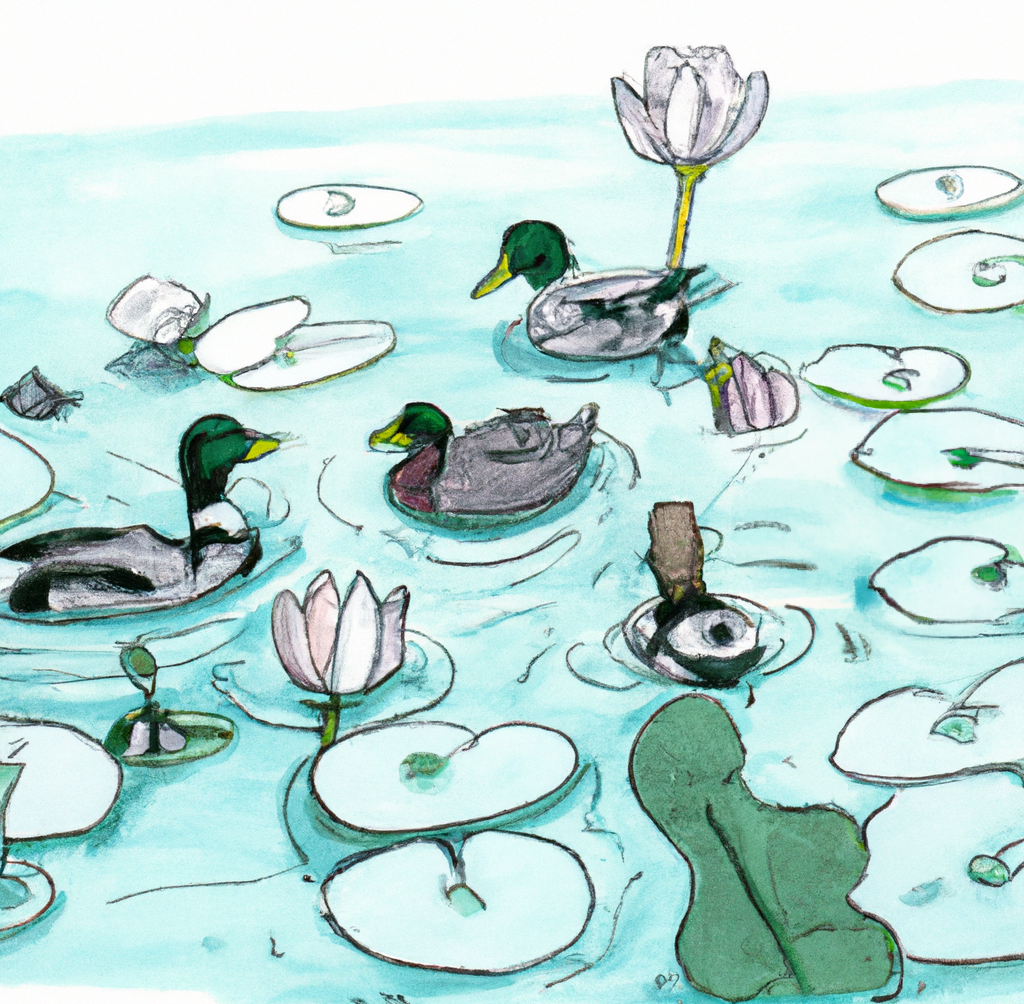
\includegraphics[width=0.35\textwidth, right]{img/dalle-ducks.png}
        \captionsetup{textformat=empty,labelformat=blank}
        \caption{Generated with Dall-E. \url{https://labs.openai.com/}. ``A duck dominating sitting on a sea rose''}
\end{figure}

\epigraph{\itshape Todo select another quote}{Lewis Caroll, \textit{XXXX}}

Quack! Quack! You are careless for a second and immediately the dreaded \textit{geesiosi} clan has taken the opportunity and conquered the \textit{Merganser Lake} by pushing away your befriended ducks!
Now they are sitting on all the beautiful water lilies without the will of giving them back and the desperate ducks have asked for your assistance.
The ducks have given you a map of the lake (see \cref{fig:duck-lake}) where all the water lilies are marked in green.
You instantly assured them of your help and started to analyze the situation!

You quickly noticed that the \textit{geesiosi} members are very frightened of the ducks' quacking. 
One single duck can free up an entire water lily and even drive away all geese on neighboring plants! After thinking about this for a few minutes you realized that this might indeed be the key observation to regain the lake. 
After some more deep contemplating, you even came up with a good assignment of ducks to water lilies, where only a minimal number of ducks is required to liberate the whole territory again.

Happy with your idea, you present it to the \textit{Supreme Duck Decision Board}, but unfortunately, you could not fully convince them and the \textit{Chief Strategy Duck} shared her worries with you: 
They know that they also have to hold the fort and protect the lake against another future rush of the \textit{geesiosi}.
This is going to be very boring for the individuals because a duck has to sit alone on a water lily waiting all day. They would rather want to have at least someone around to quack with together!

%____
You suggest them to revise your solution making sure that there is always another friend sitting at most two water lilies away. After (going back),  you came up with a new solution

They want to know what the \textit{least} number of ducks is they have to send such that all the \textit{geesiosis} are put to flight - after all, they still have other things to do and do not want to send more ducks to fight than necessary!

% FROM https://creazilla.com/nodes/41547-duck-clipart
\begin{figure}
    \centering
    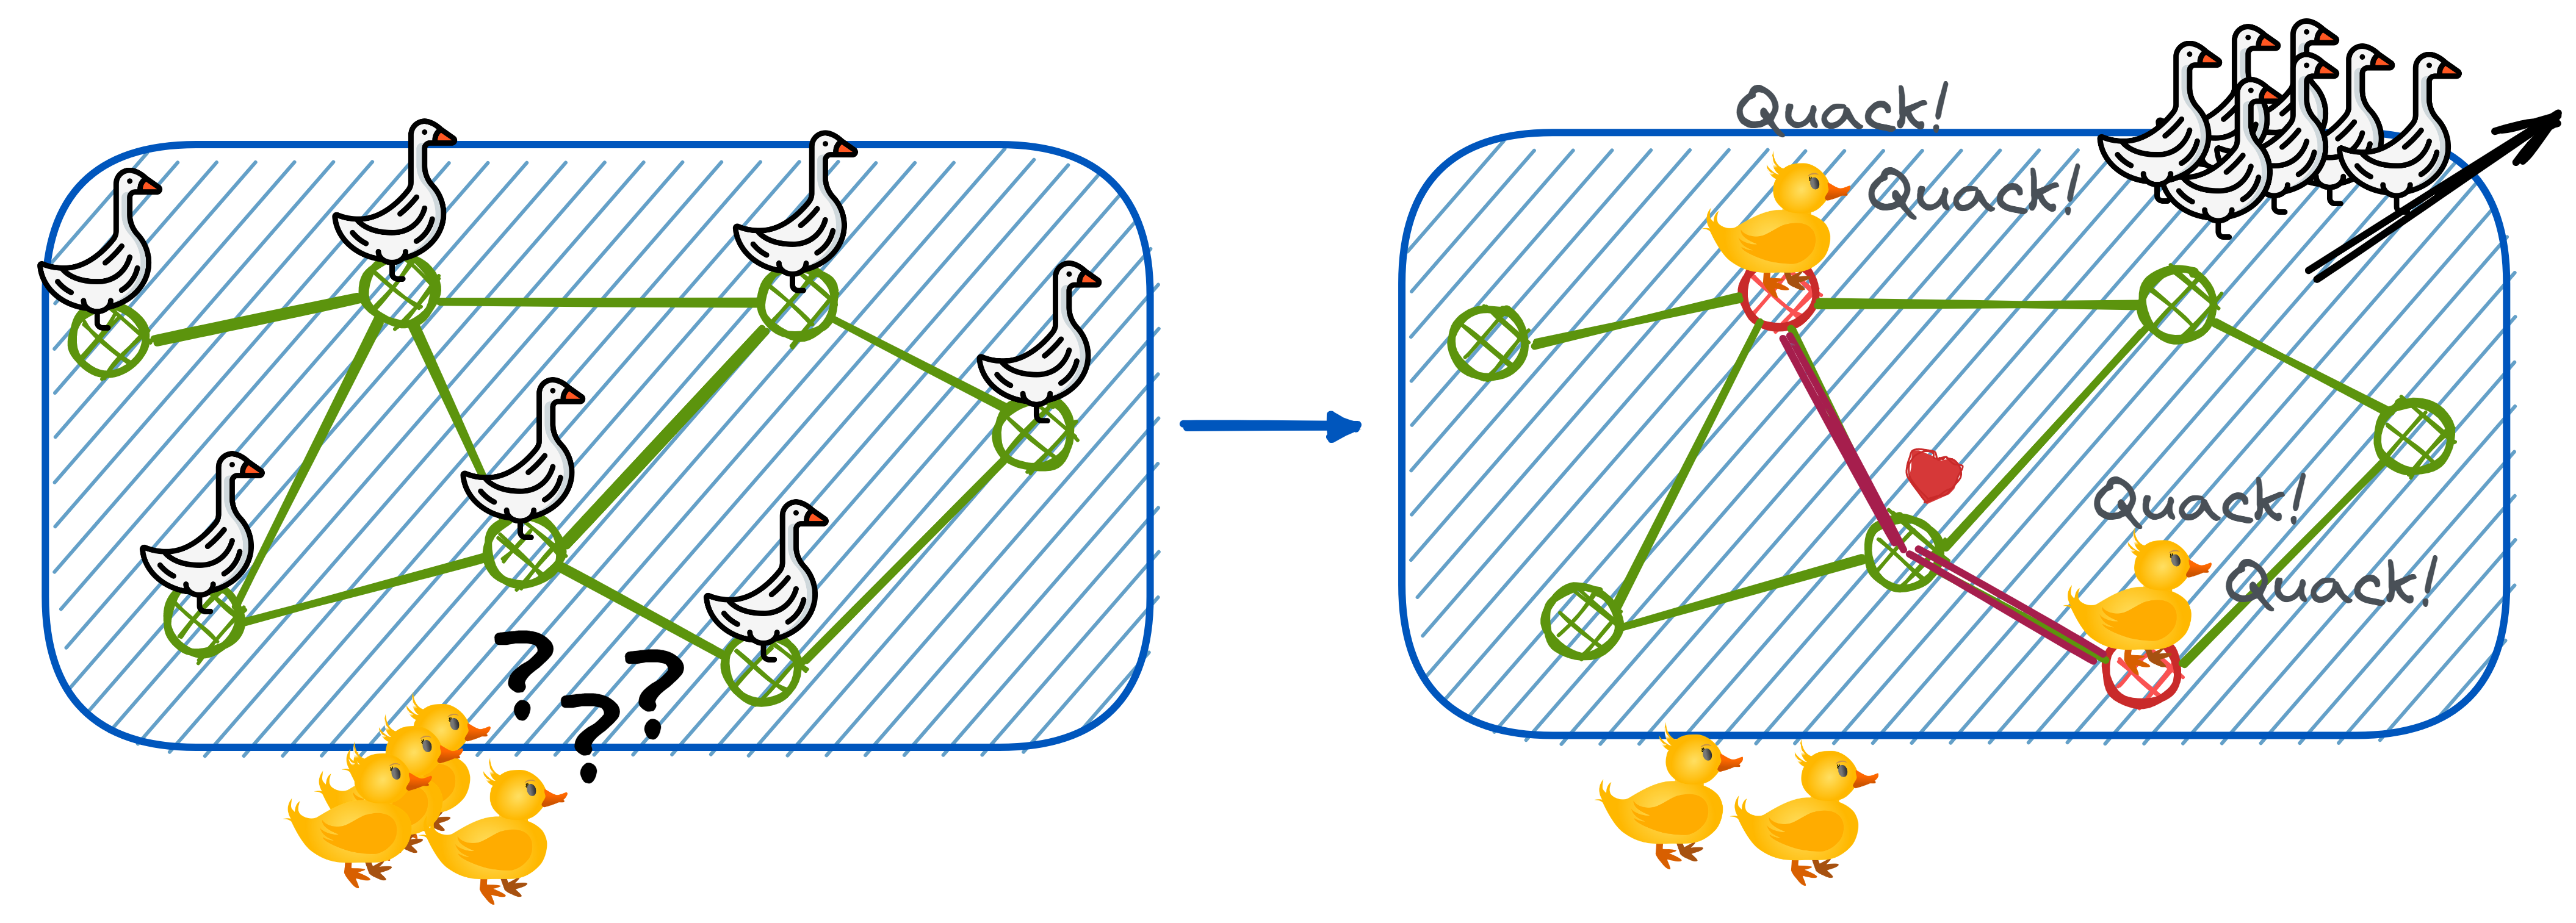
\includegraphics[width=0.9\columnwidth]{excalidraw/lake.png}
    \caption[Introductions: Merganser Lake. Own Drawing. Embedded icons under public domain from {\href{https://creazilla.com/}{https://creazilla.com/}}]{\textit{Left: All water lilies are occupied by members of the \textit{geesiosi} clan! The handwritten arrows have been your first solution proposal which was refused by the \textit{Supreme Duck Decision Board}.
    Right: Your second and final solution: Two ducks are enough to make all \textit{geesiosi}'s flee. Furthermore, they are only two water lilies apart (red line) and therefore have someone to quack together with!}}
    \label{fig:duck-lake}
\end{figure}

Can you help them? 


\textbf{Problem Definition}

\begin{prb}[DOMINATING SET {\cite[p. 586]{Cygan2015}}]{prb:ds}

    \begin{tabularx}{0.9\textwidth}{>{\hsize=0.30\hsize}X>{\hsize=0.8\hsize}X}
        \textbf{Input:} & Graph \G and an integer $k$\\
        \textbf{Question:} & Is there a set $X \subseteq V$ of size at most $k$ such that $N[X] = V$? \\
    \end{tabularx}
        
\end{prb}

\begin{prb}[SEMITOTAL DOMINATING SET {\cite{Goddard2014}}]{prb:tds}
    
    \begin{tabularx}{0.8\textwidth}{>{\hsize=0.35\hsize}X>{\hsize=0.8\hsize}X}
        \textbf{Input:} & Graph \G and an integer $k$\\
        \textbf{Question:} & Is there a subset $X \subseteq V$ of size at most $k$ such that $N[X] = V$ and for all $d_1 \in X$ there exists another $d_2 \in X$ such that $d(d_1, d_2) \leq 2$?\\
    \end{tabularx}
        
\end{prb}

\begin{prb}[TOTAL DOMINATING SET {\cite[p. 596]{Cygan2015}}]{prb:sds}
    
    \begin{tabularx}{0.8\textwidth}{>{\hsize=0.35\hsize}X>{\hsize=0.8\hsize}X}
        \textbf{Input:} & Graph \G and an integer $k$\\
        \textbf{Question:} & Does there exists a set $X \subseteq V$ of at most $k$ vertices of G such that for every $u \in V(G)$ there exists $v \in X$ with $\{u,v\} \in E$ \\
    \end{tabularx}
        
\end{prb}



\section{Content of the thesis}

In this thesis, we continue the systematic analysis of the \sdom problem by focusing on the parametrized complexity of the problem. 

Although the problem already had a lot of attention regarding classical complexity (CITE), only a few results are currently known for the parametrized variant. 

As far as we have seen, even the w-hardness of the general case has not been explicitly proven in the literature. 

In this thesis, we continue the journey toward a systematic analysis by stating some hardness results for specific graph classes for the problem.

\paragraph{Our contributions}
% TODO Better: 

Our main contributions consist of first showing the $w[2]$-hardness of \sdom for XXXX graphs.

\noindent As the \dom problem and the \tdom problem both admit a linear kernel for planar graphs, it is interesting to analyze whether these results also hold for the \sdom problem which lies in between these two. 
%TODO by relxing the witness of these two provlemsproblems.

Having these kernels also for other variants like \eddom, \efdom, \cdom, \rbdom lent us great confidence that the result will also work for \sdom on planar graphs.

%% TODO Find more  .

Following the approach from ... which already relies on the technique given in, we give some simple data reduction rules for \sdom on planar graphs leading to a linear kernel. More precisely, we are going to prove the following central theorem of this thesis:

With some modifications, we were able to transfer the approach given by Garnero and Sau in \cite{Garnero2018} to the \sdom problem.

\begin{restatable}[]{theorem}{centraltheo}\label{thm:central}
    The \sdom problem parametrized by solution size admits a linear kernel on planar graphs. There exists a polynomial-time algorithms that given a planar graph $(G, k)$, either correctly reports that $(G, k)$ is a NO-instance or returns an equivalent instance $(G', k)$ such that $\abs{V(G')} \leq \kernelsize \cdot k$.
\end{restatable}

\dom problem and \tdom problem, both already 

\begin{figure}[t]
     \begin{equation*}
         \tikzfig{fig/tikz/ds-examples}
     \end{equation*}
    \caption[An example for various dominating sets]{\textit{An example  for a \dom, \sdom and \tdom, where $\gamma(G) < \gamma_{2t}(G) < \gamma_t(G)$ are strict. In the first case, only two vertices suffice to dominate all others. In the second one, we need a witness between $d_1$ and $d_2$ that is at most distance two. In the last case, $d_1$ and $d_2$ both need a neighbor in the \tdom.}}
    \label{figd:dsexamples}
\end{figure}
